\label{ch:3}
In this section, we discuss different learning-based approaches that have been explored in recent years. \edited{To keep the discussion relevant to the contribution of the thesis, the discussion is focused on bodies work that fall under the banner of reinforcement learning (RL) or inverse reinforcement learning (IRL) based methods. Both RL and IRL have been widely researched in the field of socially-aware navigation.} While these methods differ at their core, the problem definition for both the cases is mostly similar but with a key difference. For both RL and IRL setting, the problem at hand is expressed in the form of a Markov decision process (MDP). We define the problem below.
\subsection*{Problem definition:}
A Markov decision process is a discrete-time stochastic control process and can be represented as a 5 tuple
($\mathcal{S}$,$\mathcal{A}$,T,$\gamma$, $\mathcal{R}$), where,
\begin{itemize}
    \item $\mathcal{S}$ is the set of all possible states.
    \item $\mathcal{A}$ is the set of all possible actions.
    \item T is the transition dynamics.
    \item $\gamma$ is the discount factor.
    \item $\mathcal{R}$ is the set of rewards.
\end{itemize}  
In reinforcement learning problems, the goal is to find a policy $\pi$: a function that maps a state to an action that maximizes the expected reward obtained.\\
In contrast, in inverse reinforcement learning problems, there is no reward function. Instead, a set of expert demonstrations is provided. This can be denoted by, D = \{$\tau_1$, $\tau_2$, ... \}. The goal is to generate a reward function $\mathcal{R}$, which best explains the expert behavior and a policy that maximizes the reward function.


\section{RL based approaches}
 With their remarkable success in the field of video games and a suite of tasks of similar anatomy, RL has been one of the go-to tools in the field of social navigation in recent years. \\
Chen et al. \cite{chen_socially_2017} address this problem by focusing on what not to do, rather than what to do. They introduce a reward function crafted to induce social norms in the behavior of the agent. The reward function primarily focuses on three different aspects of interaction: overtaking, passing, and crossing as shown in \autoref{fig:chen_socially_crossing}
 \begin{figure}[!htbp]
     \centering
    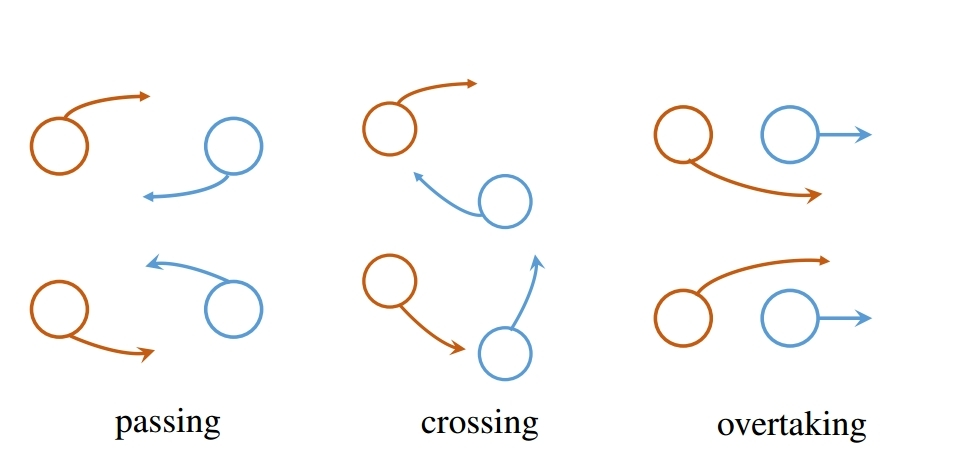
\includegraphics[width=.6\linewidth]{figures/chapter2_rl_based_approach}
    \caption{\edited{Symmetric pairwise collision avoidance in a time efficient manner by the red agent in the three interaction scenarios. The interactions in the top and bottom row are often referred as left and right-handed rules respectively.}}
    \label{fig:chen_socially_crossing}
 \end{figure}
\thcomment{In their paper they write : "This work notes that social norms are one of the many
	ways to resolve a symmetrical collision avoidance scenario,
	as illustrated in... "}
They claim that symmetry is one of the driving factors \edited{that} incorporate social behavior. The reward function they define is given by \autoref{eq:chen_socially_2017_reward_function}.
\begin{align}
\label{eq:chen_socially_2017_reward_function}
\begin{split}
R_{norm}(s^{jn}, a) &=  q_nI(s^{jn} \in S_{norm})\\
s.t. \qquad S_{norm}&=  S_{pass} \cup S_{ovtk} \cup S_{cross}\\
S_{pass} &= \{s^{jn} | d_g > 3, 1 < \tilde{p_x} < 4,
			  -2 < \tilde{p_y} < 0, |\tilde{\phi} - \psi| > 3\pi/4 \} \\
S_{ovtk} &= \{s^{jn} | d_g > 3, 0 < \tilde{p_x} < 3, |v| > |\tilde{v}|
			  0 < \tilde{p_y} < 1, |\tilde{\phi} - \psi| < \pi/4 \} \\
S_{cross} &= \{s^{jn} | d_g > 3, \tilde{d_a} < 2,  \tilde{\phi_{rot}} > 0,
			  -3\pi/4 < \tilde{\phi} - \psi < -\pi/4  \}
\end{split}
\end{align}\\
where, $I$ is an indicator function. $S_{pass}$, $S_{ovtk}$, and $S_{cross}$ are the set of states that fall under the category of passing, overtaking and crossing respectively, $s^{jn}$ is the joint state of the agent and its neighbor, $a$ is the action, $q_{n}$ is a scalar penalty, $d_{g}$ is the distance of the goal from the agent, $d_{a}$ is the distance to the neighboring agent, $\tilde{\phi}$ is the neighboring agent's orientation, $\phi$ is the agent's orientation, $\tilde{\phi_{rot}}$ is the relative rotation angle between the two agents and $\tilde{p_x}$ and $\tilde{p_y}$ are the $x$ and $y$ coordinates of the neighboring agent in the target agent's reference frame. The reward function in \autoref{eq:chen_socially_2017_reward_function} biases the agent towards adhering to the right-hand rules.
\\

A more recent work by the same authors, "Collision avoidance in pedestrian-rich environments with deep reinforcement learning" \cite{everett_collision_2019}, \thcomment{Yes, it is the title of their paper.}
address drawbacks of their previous work: the inability to tackle a variable number of agents in the environment. They introduce a \edited{long short-term memory} (LSTM) \cite{hochreiterLongShortTermMemory1997} network architecture as shown in \autoref{fig:everett_lstm_network} that takes as input the information from the nearby pedestrians in a sequence which eliminates the need for specifying a limit on the number of nearby-agents the method can handle.
\begin{figure}[!htbp]
	\centering
	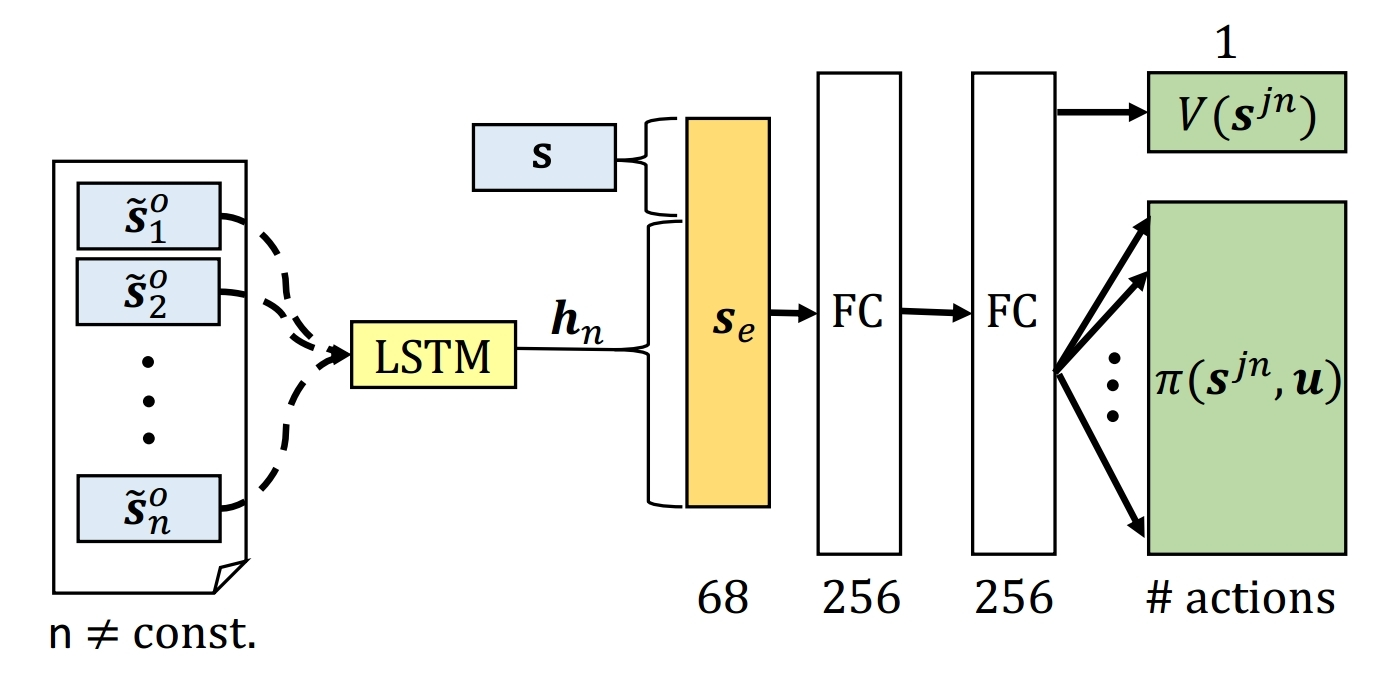
\includegraphics[width=0.6\linewidth]{figures/everett}
	\caption{LSTM based network architecture to account for a variable number of nearby agents.}
	\label{fig:everett_lstm_network}
\end{figure}
 For this work, they select a relatively simple sparse reward function that focuses on collision avoidance and maintaining distance from others as shown in \autoref{eq:everett_reward_function}\\
\begin{align}
\label{eq:everett_reward_function}
f)x) = 
\begin{cases}
	 1 & \text{if \quad $p=p_g$} \\
	 -0.1+d_{min}/2 & \text{if \quad 0 < $d_{min}$ < 0.2} \\
	 -0.25 & \text{if \quad $d_{min}$ < 0}\\
	 0 & \text{otherwise}, 
\end{cases}
\end{align}
where $d_{min}$ is the distance to the nearest neighboring agent.
%\textbf{Conclusion}\\
\subsection*{Conclusion}

\edited{Reward function is the most succinct definition of the task at hand \cite{abbeel_apprenticeshiplearning_2004}, making it a vital component that determines the final performance of a RL method. We can see similarities between RL methods and other classical approaches. RL method still involve reward engineering, which can get pretty complex even when considering a handful of simple interactions. The reward function by Everett et al. \cite{everett_collision_2019} focuses solely on collision avoidance, and Chen et al. \cite{chen_socially_2017} incorporate an element of naturalness to the mix using symmetry. But it takes into account a very limited number of scenarios: just 3 possible interaction scenarios, which is a small subset of the very many implicit intentions and explicit decisions a human takes while navigating.}
 
Reinforcement learning, as a class of methods, has been widely successful in solving various complex control tasks including, but not limited to, video games making it one of the more preferred choices to tackle the problem of social navigation. \par
Using RL in this particular setting however necessitates the formulation of a reward function that can correctly capture the 'social and cultural' characteristics. As noted earlier, coming up with such a set of rules can be difficult and daunting as 'social norms' are not always explicit and can vary widely across different societies and even based on a given situation.\\

\section{IRL based approaches}
%\textbf{Learning approaches meet probabilistic road map style path planner.}
\edited{Inverse reinforcement learning bypasses the step of engineering the reward function, instead, it aims at recovering the underlying reward function using expert demonstrations, making it an attractive alternative to RL based methods. IRL has been extensively explored to address the problem of social navigation.} \\
Vasquez et al. \cite{vasquez_inverse_2014}, present a comprehensive study on the effect of different feature representations and IRL methods on the performance of an agent in the task of social navigation. They examine two IRL methods: max-margin IRL and max-entropy IRL. \edited{Max-margin IRL aims at finding a set of weight parameters that maximizes the margin between the feature expectation of the expert demonstrations and that of the trained policy. The goal of max-entropy IRL is to find a set of weight parameters that maximizes the likelihood of the expert demonstrations, where the probability of occurrence of a given roll-out is proportional to the exponential of the reward obtained by it.} \\
For the feature representations, they create a pool of measurements garnered from the state of the agent itself and the state of the other entities in the environment and combine these measurements to create 3 feature representations. \\
They test these on a \edited{Robot Operating System or, in short, ROS-based} pedestrian simulator on 3 scenarios: airport gate, crossing hallway, and intersection. Expert demonstrations for these scenarios are obtained through tele-operation. They find that the performance across the two learning methods are similar. The feature representation, on the other hand, plays a major role in the final performance of the agent hence they come to the conclusion that spending time on modeling the feature representations or working to come up with learning methods that aid in the simplification of building the feature representations might be the way to go.
\\
\par
Kim and Pineau \cite{kim_socially_2016}, Socially adaptive path planning, present a way to automate the navigation of a wheelchair in a social setting. Their navigation framework comprises of 3 components, the feature extractor, the IRL module, and the path planner.\\
%\textbf{Feature extractor}
The features are generated from the readings of an RGB-d sensor ($3$D point cloud) mounted on the robot. The area around the agent is divided into $3$D blocks or cells and the features are calculated for each of these spatial cells. 
The authors calculate $4$ features namely,
crowd density, speed, velocity, and distance to the goal.
While the calculation of the crowd density and the distance to the goal is straight forward, the calculation of the speed and velocity from 3d point clouds are more involved and the authors use an RGB-d optical flow method based on Farneback RGB optical flow \cite{farneback_optical_flow}. 
The result is a $12$-dimensional binary feature vector for each grid cell.
%\textbf{IRL module}
The authors use maximum-a-posteriori Bayesian inverse reinforcement learning (MAP-BIRL) \cite{choi_MAP-BIRL_2011} to calculate the cost function for socially acceptable navigation. The cost of a state is given by
\begin{align}
C(s,a) &=w \cdot \phi(s,a)
\end{align}
where, $\phi(s,a)$ is the feature representation of the state $s$ and $w$ is the weight vector learned from MAP-BIRL. 
The weight vector is obtained by obtaining the maximum-a-posteriori (MAP) inference of the following expression:
\begin{align}
L(w) = \sum^M_{m=1} \sum^{H}_{h=1}log[\frac{\exp \mathcal{Q}^{*}_m(s^m_h, a^m_h)}{\sum_{a\in A} \exp(\mathcal{Q}_m^*(s_h^m,a))}]
\end{align}
\edited{where, $M$ is the number of trajectories in the expert demonstration, $H$ is the number of states in each trajectory, $s_{h}^{m}$ and  $a_{h}^{m}$ is the state observed and action taken at time step $h^{th}$ of trajectory $m^{th}$ respectively, and $\mathcal{Q}^{*}_m(s^m_h, a^m_h)$ is the cumulative discounted future reward associated with that state-action pair.}\\ 
For path planning, the authors maintain a hierarchical path planner consisting of 3 parts: a global planner, a local planner, and a collision detector.
The global planner chalks out a global path from the starting position of the robot to the goal state. The entire path is broken down into multiple sub-goals and the responsibility of moving from one sub-goal to the next falls on the local planner. During the run, the planner maintains a collision detector based on handcrafted rules.
The authors test their method on different scenarios including one that involves the robot operating in a crowded corridor.\\

Fahad et. al. \cite{fahad_learning_2018}, present a navigation framework to train agents from demonstrations using maximum entropy deep IRL where the objective is to maximize the likelihood of the states visited by the expert.
This is achieved by dividing each demonstration, or trajectory, in this case, into a sum of the individual states encountered by the expert. and minimizing the difference in the state visitation frequency (SVF) of the agent and the expert.\\
The authors present a feature representation consisting of 4 parts:
\begin{enumerate}
    \item Social Affinity Map(SAM): This captures the motion of the pedestrians in the vicinity of the agent. The area near the agent is divided into two concentric circles. The region inside the inner circle is then divided into 4 parts, and the region between the inner and outer circle is divided into 6 parts as shown in \autoref{fig:SAM_local_bins}
    Information from each of these 10 areas (or bins) is then expressed using a 6-dimensional vector that captures the average velocity of the pedestrians in a given bin. 
    \begin{figure}
    	\centering
    	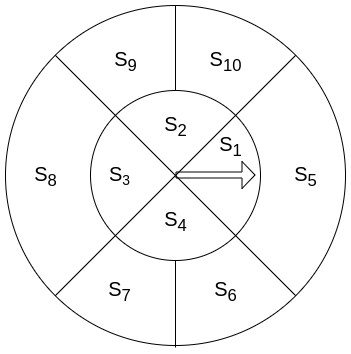
\includegraphics[width=0.5\linewidth]{figures/SAM_local_bins.png}
    	\caption{Division of the area around the agent into spatial bins as done in the SAM features. The arrow marks the direction of heading of the agent.}
    	\label{fig:SAM_local_bins}
    \end{figure}
    \item Density feature: Helps provide an idea of how dense the vicinity of the agent is. It is calculated by adding up the number of pedestrians present in the spatial bins (calculated above). Once calculated they are discretized based on some predefined threshold.
    \item Distance feature: Captures the distance between the agent's current location and the goal.
    \item Default Cost feature: Introduced to balance the rest of the other features. This has been proposed by various other works in the past.
    
\end{enumerate}
The authors train and test their procedure using data collected in the "ATC" business center in Osaka, Japan.
From these experiments, they show that the method is not only capable of producing a general navigator to negotiate the crowd, but also an agent that show traits of pedestrian behaviors like collision-avoidance and following the leader.


\subsection*{Conclusion}
\edited{Both Vasequez et al. \cite{vasquez_inverse_2014} and Fahad et al. \cite{fahad_learning_2018} assume availability of the transition dynamics of the environment which is difficult to obtain in a real-world environment. They also test their models on fairly restrictive scenarios. Vasquez et al. test on 3 specific interaction scenarios: an airport gate, a crossing hallway and an intersection, and, Fahad et al. select a section of a corridor inside a mall. While it represents data taken from actual pedestrians instead of simulation, they lack the richness of human interaction that comes from an open space that puts minimal restriction on the flow of the crowd. Kim et al. \cite{kim_socially_2016} take a different approach and use a layered control architecture, each responsible for a specific part of the navigation. It is unclear as to how much the different control modules interfere in each other's decision and how this affects the overall performance of the method. For example, in an overcrowded environment if the collision detector module keeps over ridding control from the the local planner, then what percentage of the resulting trajectory will be the output of the collision-avoidance module compared to that of the IRL planner.}
\par
Given the nature of the task, IRL based methods seem to be a promising avenue to explore. But the problem of social navigation is far from solved and many issues still need addressing. IRL methods are highly dependent on the design of the feature representation used in the algorithm, and a lot of time and effort are needed towards optimizing a set of features that would perform well. Moreover, for most of the existing work, not a lot has been discussed about the generalization of the agent. Most of the experiments are either conducted in a relatively simple environment, like a narrow hallway, or address some specific aspect of crowd navigation like negotiating intersections.
\begin{comment}
\textbf{Collection of expert trajectory might be expensive}
\textbf{The generalization of the method is not that great for now}
\textbf{The dependence of IRL on feature engineering: IRL methods are highly dependent on the design of the feature representation used in the algorithm, and a lot of time and effort are needed towards optimizing a set of features that would perform well.}

The primary advantage of IRL over the other methods discussed, both model-based and data-driven methods, is that there is no need to specify a handcrafted reward function built to induce certain kinds of behavior within the agent. Most of the current work in this domain primarily focuses on capturing the expert's behavior, thus encapsulating the 'naturalness' in the movements during navigation.
Disadvantages:
Comment of IRL and feature engineering. 
Getting expert demonstrations are more expensive compared to RL.
Hard to generalize. 
\end{comment}